\section{Supplementary evidence and reproducibility}
This Supplement retains complete development studies and their limits. It
does not reinterpret exploratory results as held-out confirmation.

\subsection{Architecture, matcher and training details}
D1 has one query-only cross-attention block with four heads of width 32 and
a 128-dimensional feed-forward bottleneck. Candidate descriptors are unchanged.
A LayerNorm--MLP scalar head of hidden width 64 adds a bounded
$0.25\tanh$ residual to contextual cosine. The listwise objective averages
eligible queries within an asset; assets without an eligible query do not
update the matcher. The final seven-pass checkpoint contains 62,545 updates,
using AdamW rate $10^{-4}$, weight decay 0.01 and gradient clipping 1. Six
teacher-rejected cases affect matcher training only; the SS population is
still 9,149. No test matching-head training or calibration is performed.

The selected SS uses identity values and no new learned readout. An evaluated
alternative anchors learned logit refinement to its initial score:
\begin{equation}
 a_{rhk}=\operatorname{softmax}_{k\in\mathcal K_r}
 [\log p_r(k)+s_{rhk}(\theta)-s_{rhk}(\theta_0)].
\end{equation}
Four-head probabilities average before native value aggregation. Prior-weighted
centering of the score difference preserves this softmax, and zero prior
support remains zero. This initialization reproduces Fixed weights, but an
initialization safeguard is not evidence of a quality advantage. Learned
V/output transforms are distinct alternatives. Absent deformation-query
channels and source modules are physically removed in their respective
controls.

The original SS/PBR base and frozen matcher tensors, LoRA initialization,
per-rank input/noise/timestep traces, and saved checkpoint/config hashes are
verified in the experimental artifacts. Main SS comparisons use a native
microbatch 96 without accumulation; native PBR uses four ranks with
microbatch 6, accumulation 1 and global batch 24. Shape stages, image encoders,
Omega and the matching decoder remain frozen during generative fine-tuning.

\subsection{Original module family and independent training}
\input{typeset/dev-ss128.tex}
\input{typeset/dev-original-module-effects.tex}
\input{typeset/dev-independent-ss.tex}
The original 12-model family has ten prespecified module contrasts; its
adjusted intervals include zero. Two follow-up evidence designs are reported
separately. In the original FULL family, ray minus voxel macro IoU is
$-0.000236$, with adjusted interval $[-0.000878,0.000351]$. Member minus mean
is$-0.000601$, with $[-0.002246,0.001262]$. These results do not establish a
positive quality effect or equivalence, and the original learned readout is
not the selected Fixed architecture.

The two-seed SS study uses 4,000 source-cluster draws for three IoU contrasts
separately within each seed and for the fixed-two-checkpoint mean. It is not
a simultaneous nine-comparison or training-seed-population interval. Fixed
minus V1 is positive in both actual runs; Fixed minus Top-1 remains uncertain.
For selected Fixed SS, two fresh VAL36 loads verify latent/occupancy
consistency and tail-batch behavior before TEST. The V1/Top-1 controls retain
their own archived checkpoint-binding and native parity checks; these are
not a two-fresh-load study of all seven ablation checkpoints.

\input{typeset/dev-independent-pbr.tex}
The two-seed PBR training diagnostic retains each producer's fixed-four
GT-shape target reference and declared initial-render policy. Across seeds,
input RGB, cameras, noise and initial latent checks are exact, but these
curves are not pooled as common-pixel source-preservation evidence.

\subsection{Paired geometric and appearance studies}
\input{typeset/dev-geometry-contrasts128.tex}
\input{typeset/dev-completed-fixed-contrasts.tex}
\input{typeset/dev-joint32.tex}
\input{typeset/dev-joint128.tex}
\input{typeset/dev-pbr-appearance32.tex}
\input{typeset/dev-paired-pbr32.tex}
All 48 downstream family values are retained unrounded in the source-bound
artifact. The displayed geometric intervals use that complete correction;
the separate SS diagnostic family averages three noises per asset. The
historical V1-geometry PBR table and the same-selected-Fixed table in the Main
text describe different fixed geometries. Their points are not exchanged or
pooled. Generated-geometry appearance and geometry results remain distinct
from fixed-GT-shape training diagnostics.

\subsection{Matching evidence and its limits}
\input{typeset/dev-matching32.tex}
\input{typeset/dev-ray-evidence.tex}
On 31,408 native observable Top-1-miss/Top-K-hit relations, mean GT mass is
1.6266\% for post-hoc Uniform, 6.4601\% for Fixed, and 6.1756\% for learned
refinement. The learned-minus-Fixed interval includes zero. Candidate
diagnostics and a relationship's stored annotation do not establish a
population quality gain or a visibility calibration. The illustration is
selected by the original conditional lexicographic rule, not downstream
render quality. Post-hoc Uniform mass is not the matched Uniform training arm.

\subsection{Full-frame and foreground sensitivity}
The primary table retains full-frame metrics. The existing producer also
reports foreground PSNR and GT-only-crop DreamSim/CLIP, with common GT-defined
crops across models. These reveal sensitivity to foreground/background
composition without model-specific recentering or alignment. They are
supplementary descriptive endpoints, not a new primary family.
\ifFinalReportReady
\begin{table*}[t]
\centering\scriptsize
\setlength{\tabcolsep}{4pt}
\begin{tabular}{lrrrr}
\toprule
\multicolumn{5}{l}{A. Source appearance: full frame and common GT-defined crop}\\
Model&DreamSim full$\downarrow$&DreamSim crop$\downarrow$&CLIP full$\uparrow$&CLIP crop$\uparrow$\\
\midrule
Zero-shot, source-only RGB4&0.153975&0.184780&0.943278&0.934490\\
Zero-shot, edited target + source RGB3&0.154276&0.186046&0.942090&0.935730\\
Vanilla V1&0.151460&0.184041&0.942854&0.937057\\
Top-1 R&0.151162&0.183377&0.943177&0.936402\\
Selected model&0.152069&0.183833&0.943018&0.935886\\
\midrule
\multicolumn{5}{l}{B. Pixel alignment: full frame and alpha-union foreground}\\
Model&\shortstack{Source PSNR\\full$\uparrow$}&\shortstack{Source PSNR\\foreground$\uparrow$}&\shortstack{Target PSNR\\full$\uparrow$}&\shortstack{Target PSNR\\foreground$\uparrow$}\\
\midrule
Zero-shot, source-only RGB4&23.17341&11.74087&22.40621&10.94126\\
Zero-shot, edited target + source RGB3&23.46619&11.90479&23.54157&11.78260\\
Vanilla V1&23.62321&12.05047&23.83599&12.06429\\
Top-1 R&23.70646&12.11024&23.99656&12.18422\\
Selected model&23.71804&12.11966&24.02827&12.21706\\
\bottomrule
\end{tabular}
\caption{Existing supplementary scores for the complete frozen TEST508 pipelines. Source means use cameras9/10; target means use camera8. Crops use the common GT-alpha bounding box with10\% padding. Foreground PSNR uses the union of predicted/GT alpha$>0.5$ and can have output-specific support. These descriptive composed-pipeline sensitivities do not isolate a PBR effect, change the primary family, or reselect a checkpoint.}
\label{tab:final-foreground}
\end{table*}

\begin{table*}[t]
\centering\scriptsize
\begin{tabular}{llrrl}
\toprule
Contrast&Endpoint&Difference&Family-adjusted95\% interval&Interpretation\\
\midrule
Selected minus Vanilla V1&LPIPS&-0.001044&$[-0.001715,-0.000446]$&benefit supported\\
Selected minus Vanilla V1&DreamSim&0.000609&$[-0.002974,0.003841]$&uncertain\\
Selected minus Vanilla V1&CLIP&0.000164&$[-0.002010,0.002200]$&uncertain\\
Selected minus Vanilla V1&PSNR&0.1923&$[0.0703,0.3201]$&benefit supported\\
Selected minus Vanilla V1&SSIM&0.001156&$[0.000538,0.001833]$&benefit supported\\
Selected minus Vanilla V1&M-IoU&0.012041&$[0.005487,0.021451]$&benefit supported\\
Selected minus Vanilla V1&CD&-0.0005139&$[-0.0014386,0.0000208]$&uncertain\\
Selected minus Vanilla V1&F-Score&0.006059&$[-0.000676,0.013572]$&uncertain\\
Selected minus Top-1 R&LPIPS&-0.000129&$[-0.000530,0.000291]$&uncertain\\
Selected minus Top-1 R&DreamSim&0.000907&$[-0.001656,0.003761]$&uncertain\\
Selected minus Top-1 R&CLIP&-0.000159&$[-0.002212,0.001829]$&uncertain\\
Selected minus Top-1 R&PSNR&0.0317&$[-0.0653,0.1267]$&uncertain\\
Selected minus Top-1 R&SSIM&0.000237&$[-0.000321,0.000673]$&uncertain\\
Selected minus Top-1 R&M-IoU&0.002863&$[-0.000239,0.008191]$&uncertain\\
Selected minus Top-1 R&CD&-0.0000233&$[-0.0001668,0.0000903]$&uncertain\\
Selected minus Top-1 R&F-Score&-0.000226&$[-0.003362,0.002879]$&uncertain\\
\bottomrule
\end{tabular}
\caption{All predeclared selected-versus-control primary comparisons, using the existing source-cluster-adjusted intervals. Source LPIPS/DreamSim/CLIP use9/10; target PSNR/SSIM/M-IoU use8; CD/F-Score use generated surfaces. Values are rounded for display; interpretation uses the original unrounded intervals and metric directions. An interval containing zero does not prove equivalence. FID/KID remain descriptive and are not included in this inferential family.}
\label{tab:final-adjusted-contrasts}
\end{table*}

\else
The actual final foreground table and 16 adjusted primary comparisons are
pending complete frozen ten-metric collection.
\fi

\subsection{Qualitative selection and remaining examples}
The original metadata declaration fixes two examples from distinct sources
without candidate scores. The first is placed in the Main text; the second
and every conditional lower-median example are included here. Empty categories
remain empty and overlapping categories share one panel. Category counts
describe eligibility, not population success rates. Images reuse exactly the
scored float arrays and official uint8 conversion, with target8/source9/10,
common M1 original-material references, and no model-specific crop or rerender.
\ifFinalReportReady
\paragraph{Predeclared conditional eligibility.}
joint-improvement: 77 eligible. The selected lower-median example appears in Fig.~\ref{fig:final-qualitative-03}.
geometry-loss: 191 eligible. The selected lower-median example appears in Fig.~\ref{fig:final-qualitative-04}.
appearance-loss: 153 eligible. The selected lower-median example appears in Fig.~\ref{fig:final-qualitative-05}.
Overlapping conditions share one panel. The first outcome-blind panel stays in the Main text even when it also satisfies a conditional category; it is referenced here rather than duplicated.
\begin{figure*}[!t]
\centering
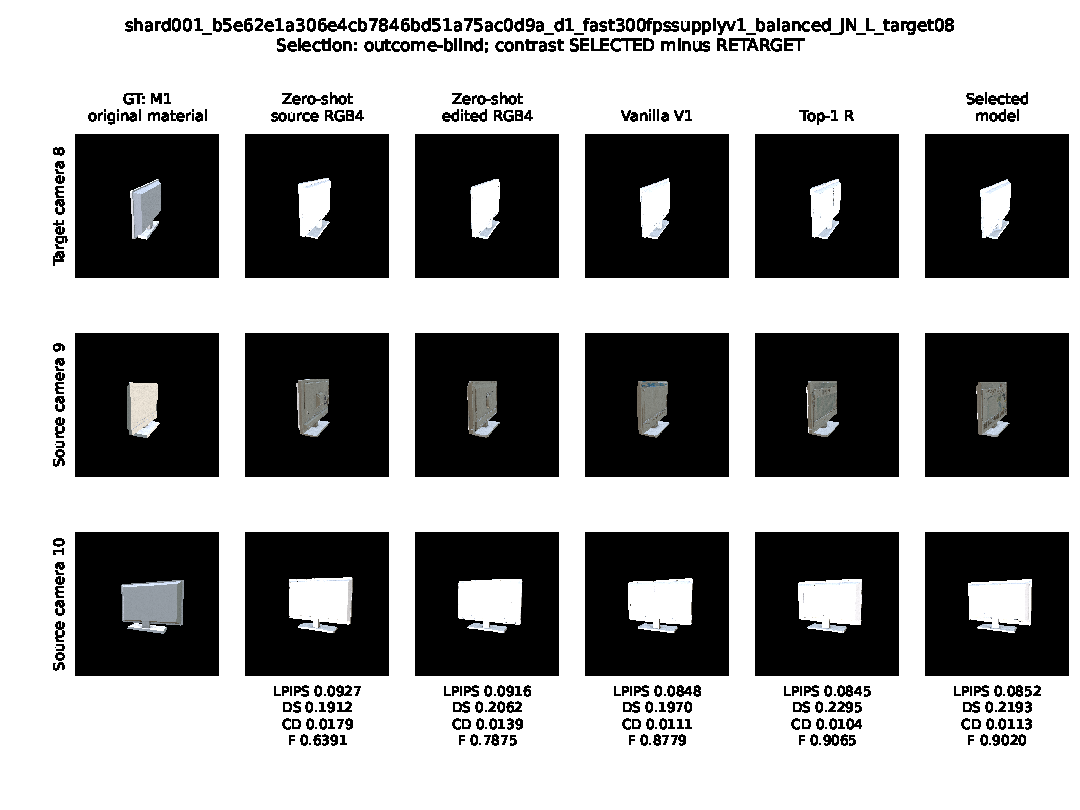
\includegraphics[width=\textwidth]{final-results/figures/example-02.pdf}
\caption{Actual scored frozen TEST example. Rows are target8/source9/source10; columns are the common original-material M1 reference and every frozen model. Selection: outcome-blind. Full-frame panels use the scored archive and official uint8 conversion, without model-specific crop, alignment or rerender. Source annotations use cameras9/10. Conditional categories illustrate their stated conditions and do not estimate population success rates.}
\label{fig:final-qualitative-02}
\end{figure*}
\begin{figure*}[!t]
\centering
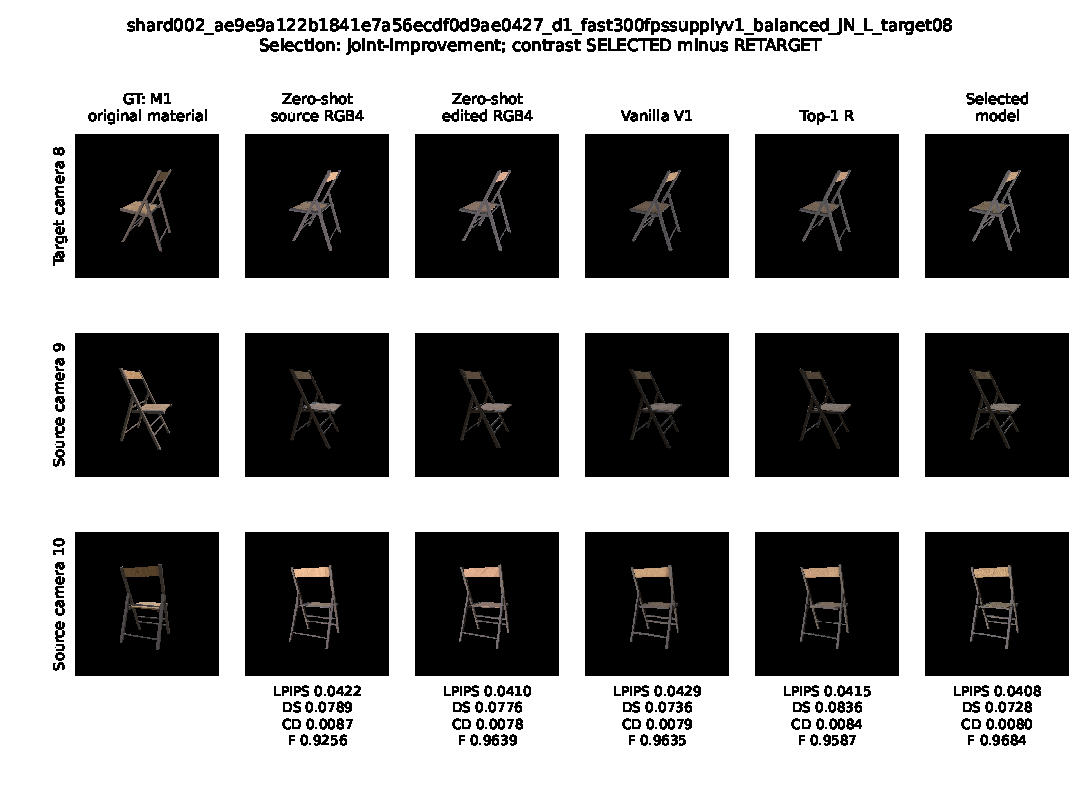
\includegraphics[width=\textwidth]{final-results/figures/example-03.pdf}
\caption{Actual scored frozen TEST example. Rows are target8/source9/source10; columns are the common original-material M1 reference and every frozen model. Selection: joint-improvement. Full-frame panels use the scored archive and official uint8 conversion, without model-specific crop, alignment or rerender. Source annotations use cameras9/10. Conditional categories illustrate their stated conditions and do not estimate population success rates.}
\label{fig:final-qualitative-03}
\end{figure*}
\begin{figure*}[!t]
\centering
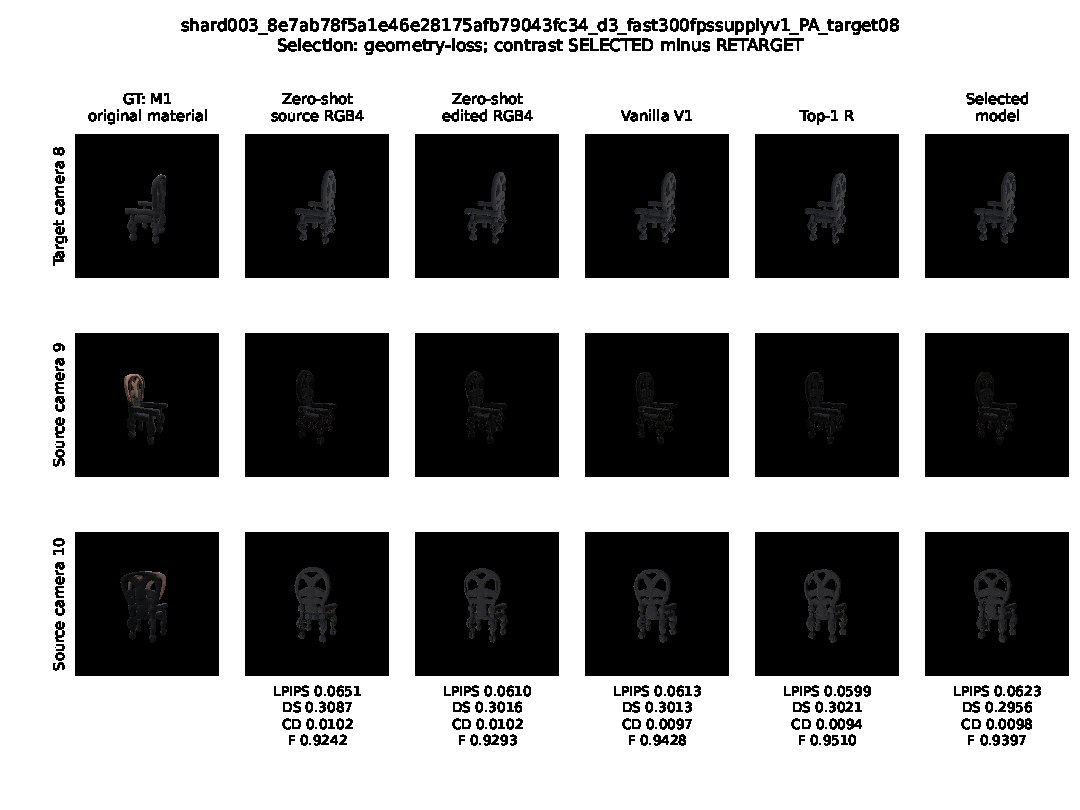
\includegraphics[width=\textwidth]{final-results/figures/example-04.pdf}
\caption{Actual scored frozen TEST example. Rows are target8/source9/source10; columns are the common original-material M1 reference and every frozen model. Selection: geometry-loss. Full-frame panels use the scored archive and official uint8 conversion, without model-specific crop, alignment or rerender. Source annotations use cameras9/10. Conditional categories illustrate their stated conditions and do not estimate population success rates.}
\label{fig:final-qualitative-04}
\end{figure*}
\begin{figure*}[!t]
\centering
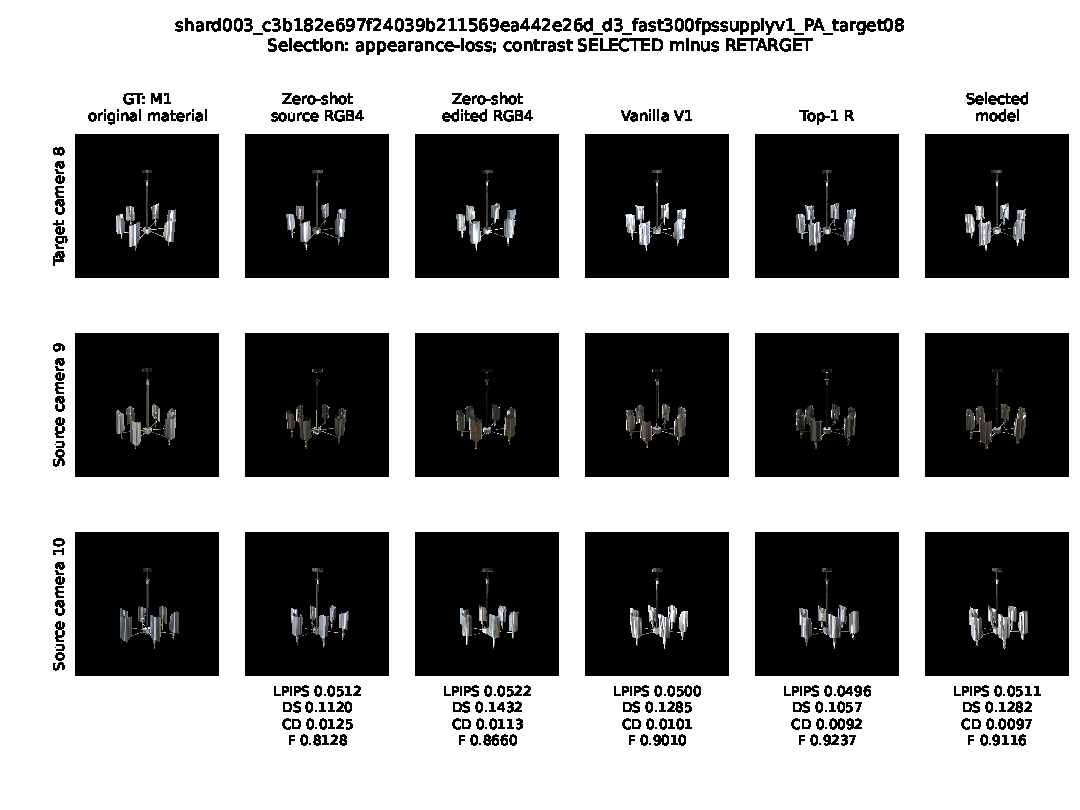
\includegraphics[width=\textwidth]{final-results/figures/example-05.pdf}
\caption{Actual scored frozen TEST example. Rows are target8/source9/source10; columns are the common original-material M1 reference and every frozen model. Selection: appearance-loss. Full-frame panels use the scored archive and official uint8 conversion, without model-specific crop, alignment or rerender. Source annotations use cameras9/10. Conditional categories illustrate their stated conditions and do not estimate population success rates.}
\label{fig:final-qualitative-05}
\end{figure*}

\fi

\subsection{Execution and reproducibility scope}
All 5 fixed pipelines use 508 test examples from 134 source clusters and one
prescribed generation noise per example. Global occupancy ratios are
distinguished from mean per-asset IoU. All 2,540 SS archives are checked for
actual latent hashes, packed occupancy and TP/FP/FN consistency; occupancy is
not substituted for surface CD/F-Score or appearance metrics. Generated
geometry is not aligned independently per output. PBR comparisons retaining
the same geometry use identical original guide values/order/scale and
rendering triangles.

The test campaign bounds complete-asset credits and retires only local raw
duplicates after every declared consumer completes and fresh canonical
file-server SHA/size checks pass. Scored images, guides, reports, source
assets and weights are retained. An initial storage-connection metadata
omission caused a controlled stop; the recovered namespace retains the same
frozen model/numerical protocol and SS inputs. Operational reader-ledger
transactions are serialized without signalling GPU workers. Such recovery
does not constitute a new model or a test-driven hyperparameter choice.
The final metric and qualitative artifacts retain actual producer/file hashes
and the original model-freeze/declaration lineage.
